%%
% Please see https://bitbucket.org/rivanvx/beamer/wiki/Home for obtaining beamer.
%%
\documentclass[handout]{beamer} % you can delete [handout] 
\mode<presentation> % change it to presentation model, but it does not work with [handout] option 
\usepackage[T1]{fontenc} 
\usepackage[utf8]{inputenc}
\usepackage{natbib}
\usepackage{amsmath}
\usepackage{amssymb}
\usepackage{graphicx}
\usepackage{etoolbox} % adjust the space before and after figure 
\usepackage{hyperref}
\usepackage{url}

\usepackage{courier} % font for code in text 
\usepackage{bm} % bold math symbol 

\usepackage{listings}
\usepackage{wasysym}
\usepackage{amsthm} % for theorem definition style 

\usepackage{rotating} % for the horizontal page table

% \usepackage{enumitem} % never use this package for beamer  

\usepackage{tikz}
\usetikzlibrary{calc}
\usetikzlibrary{matrix}
\usetikzlibrary{positioning}
\usepackage{color}
\usepackage{setspace}
\usepackage{marvosym} % symbol package 

\usepackage{booktabs} % toprule table 

\usepackage{bm} % bold math symbol 

\usepackage{bibentry}
\nobibliography*
 
\usepackage{listings}

% select the theme and color 
\usetheme{Boadilla}
\usecolortheme{beaver}

\lstset{language=Matlab}

\definecolor{mygreen}{rgb}{0,0.6,0}
\definecolor{mygray}{rgb}{0.5,0.5,0.5}
\definecolor{mymauve}{rgb}{0.58,0,0.82}

\lstset{ 
  backgroundcolor=\color{white},   % choose the background color; you must add \usepackage{color} or \usepackage{xcolor}; should come as last argument
  basicstyle=\footnotesize,        % the size of the fonts that are used for the code
  breakatwhitespace=false,         % sets if automatic breaks should only happen at whitespace
  breaklines=true,                 % sets automatic line breaking
  captionpos=b,                    % sets the caption-position to bottom
  commentstyle=\color{mygreen},    % comment style
  deletekeywords={...},            % if you want to delete keywords from the given language
  escapeinside={\%*}{*)},          % if you want to add LaTeX within your code
  extendedchars=true,              % lets you use non-ASCII characters; for 8-bits encodings only, does not work with UTF-8
  frame=single,	                   % adds a frame around the code
  keepspaces=true,                 % keeps spaces in text, useful for keeping indentation of code (possibly needs columns=flexible)
  keywordstyle=\color{blue},       % keyword style
  language=Matlab,                 % the language of the code
  morekeywords={*,...},            % if you want to add more keywords to the set
  numbers=left,                    % where to put the line-numbers; possible values are (none, left, right)
  numbersep=5pt,                   % how far the line-numbers are from the code
  numberstyle=\tiny\color{mygray}, % the style that is used for the line-numbers
  rulecolor=\color{black},         % if not set, the frame-color may be changed on line-breaks within not-black text (e.g. comments (green here))
  showspaces=false,                % show spaces everywhere adding particular underscores; it overrides 'showstringspaces'
  showstringspaces=false,          % underline spaces within strings only
  showtabs=false,                  % show tabs within strings adding particular underscores
  stepnumber=2,                    % the step between two line-numbers. If it's 1, each line will be numbered
  stringstyle=\color{mymauve},     % string literal style
  tabsize=2,	                   % sets default tabsize to 2 spaces
  title=\lstname,                  % show the filename of files included with \lstinputlisting; also try caption instead of title
  belowcaptionskip= 1 ex,
  belowskip = 1 ex
}



\title[]{Effective Computing in Research}
\subtitle{Introduction to programming and coding setup}


\author []% (optional, for multiple authors)
{Michael \inst{} \inst{}}


 
\date[] %[January 2019] (optional)
{Konstanz, March 2019}
 
\begin{document}

\begin{frame}[noframenumbering]
  \titlepage
\end{frame}

\begin{frame}{Roadmap}
	\tableofcontents
\end{frame}



\section{Introduction}

\begin{frame}{Introduction}
	This lecture aims to help people like me to setup the programming and coding environment for their own purposes. With the existence of asymmetric information, We might think programming or coding is super difficult or even have no ideas what's going on there. Therefore, I would try to do:
\begin{itemize}
	\item Give a brief on what is computing 
	\item Introduce some productivity tools for getting into the programming world
	\item Show how to setup IDEs
	\item Explain for what kind of purposes, we should learn R, Python, Matlab or even Julia, Java...etc
\end{itemize}
\end{frame}



\section{Geek Stuff}

\begin{frame}{What is computer Science}
	I used to think that computer science is kind of engineer subject. Now, I realized that this is wrong in most cases. A major portion of computer science, perhaps the most important portion, is not concerned with writing computer code. Instead, it deals with \textit{developing as well as analyzing and evaluating the algorithms} that are then implemented in computer code. 
\begin{itemize}
\setlength\itemsep{1em} 
	\item Option 1: Solve a benchmark set of linear programming problems with today’s algorithms on a machine from 1991
	\item Option 2: Solve a benchmark set of linear programming problems with 1991 algorithms on today’s machine 
\end{itemize}

Which option would you choose supposed we had a competition ?
\begin{table}[H]
	\centering
	\begin{tabular}{c|c}
	\hline
	\hline 
		Option 1 & Option 2 \\
		\hline 
		Algorithm(2000s) and Laptop(1991) & Algorithms(1991) and Laptop(2000s) \\
		\hline 
	\end{tabular}
	\caption{Optimization progress comparison from \cite{bixby2012brief}  }
\end{table}
\end{frame}


\begin{frame}{What is computer Science}
\begin{itemize}
\setlength\itemsep{1em} 
	\item \textbf{Answer:} Option 1 would be faster by a factor of approximately 300.
	\item Compared to 1980s, solving a benchmark set of linear programming problems has gain 43 million-fold speedup. Of this speedup, however, only about \textbf{1,000-fold} obtained because of Moore's law; the other \textbf{43,000-fold} obtained because of improvements in algorithms. 
	\item According to \cite{bixby2012brief}, between 1991 and 2008 the improvements arising from better algorithms and implementations have resulted in about a 29,000-fold seepdup holding the hardware at constant. 
	\item Your smartphone is millions of times more powerful than all of NASA’s combined computing in 1969. But can we send our friends to the Moon with our smartphone?
\end{itemize} 
	
\end{frame}


\section{Productivity Tools}


\begin{frame}{Get used to Terminal}
	Please, don't be terrified by this black terminal window:
	\begin{figure}[H]
		\centering
		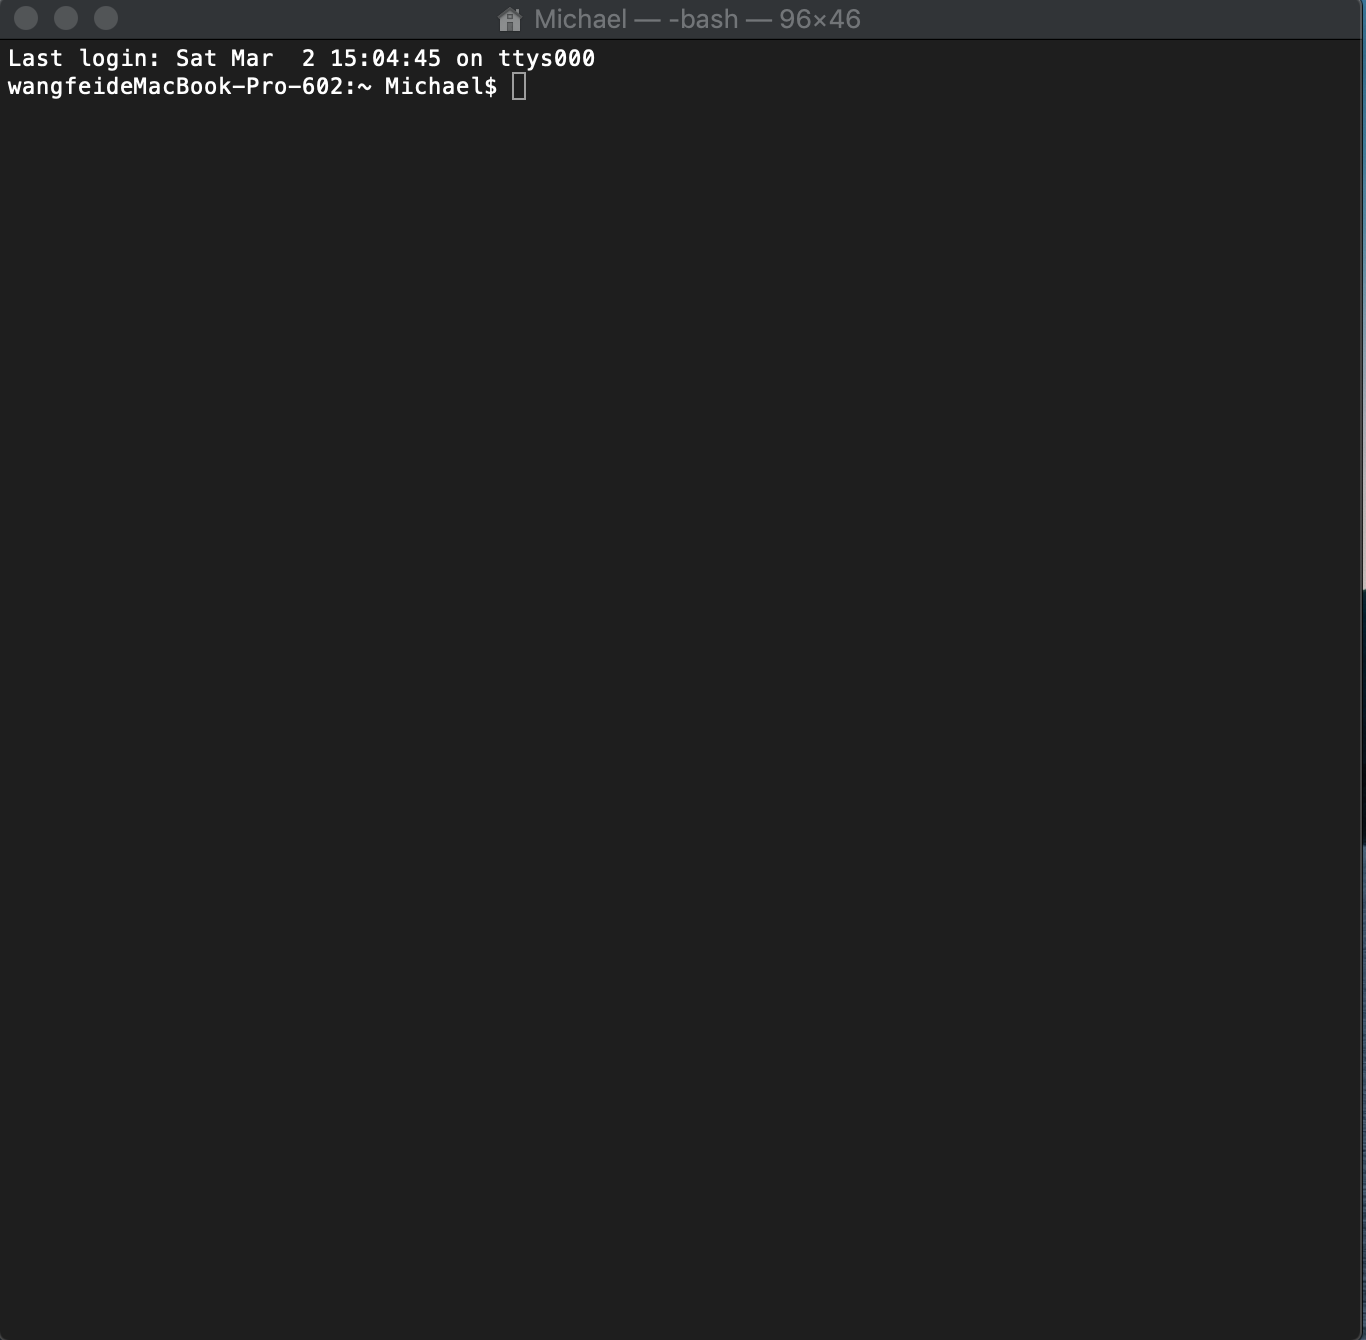
\includegraphics[width = 0.5\textwidth]{Pictures/terminal}
		\caption{Terminal on Mac}
	\end{figure}
\end{frame}

\begin{frame}{Get used to Terminal}
\footnotesize
\begin{table}[H]
	\centering
	\begin{tabular}{llc}
	\hline 
	\hline 
		Command & Function & Tips \\
		\hline 
		\texttt{pwd} & print the working directory & \\
		\texttt{man} & manual pages for the command & \\
		\texttt{Q} & quit the current section, e.g. manual & \\
		\texttt{ls} & list directory contents & \texttt{ls -a} \\
		\texttt{\~} & shorthand for the home directory & \\
		\texttt{cd} & change directory & type one space after \texttt{cd} \\
		\texttt{mkdir} & create directories (or make a file) & with path or without path \\
		\texttt{rm} & delete(or remove) files & with path or without path \\
		\texttt{cp} & copy files & \\
		\hline
	\end{tabular}
	\caption{Essential Terminal Command}
\end{table}	

\end{frame}

\begin{frame}{Get used to Terminal}
	You can customize your terminal like this:
	\begin{figure}[H]
		\centering
		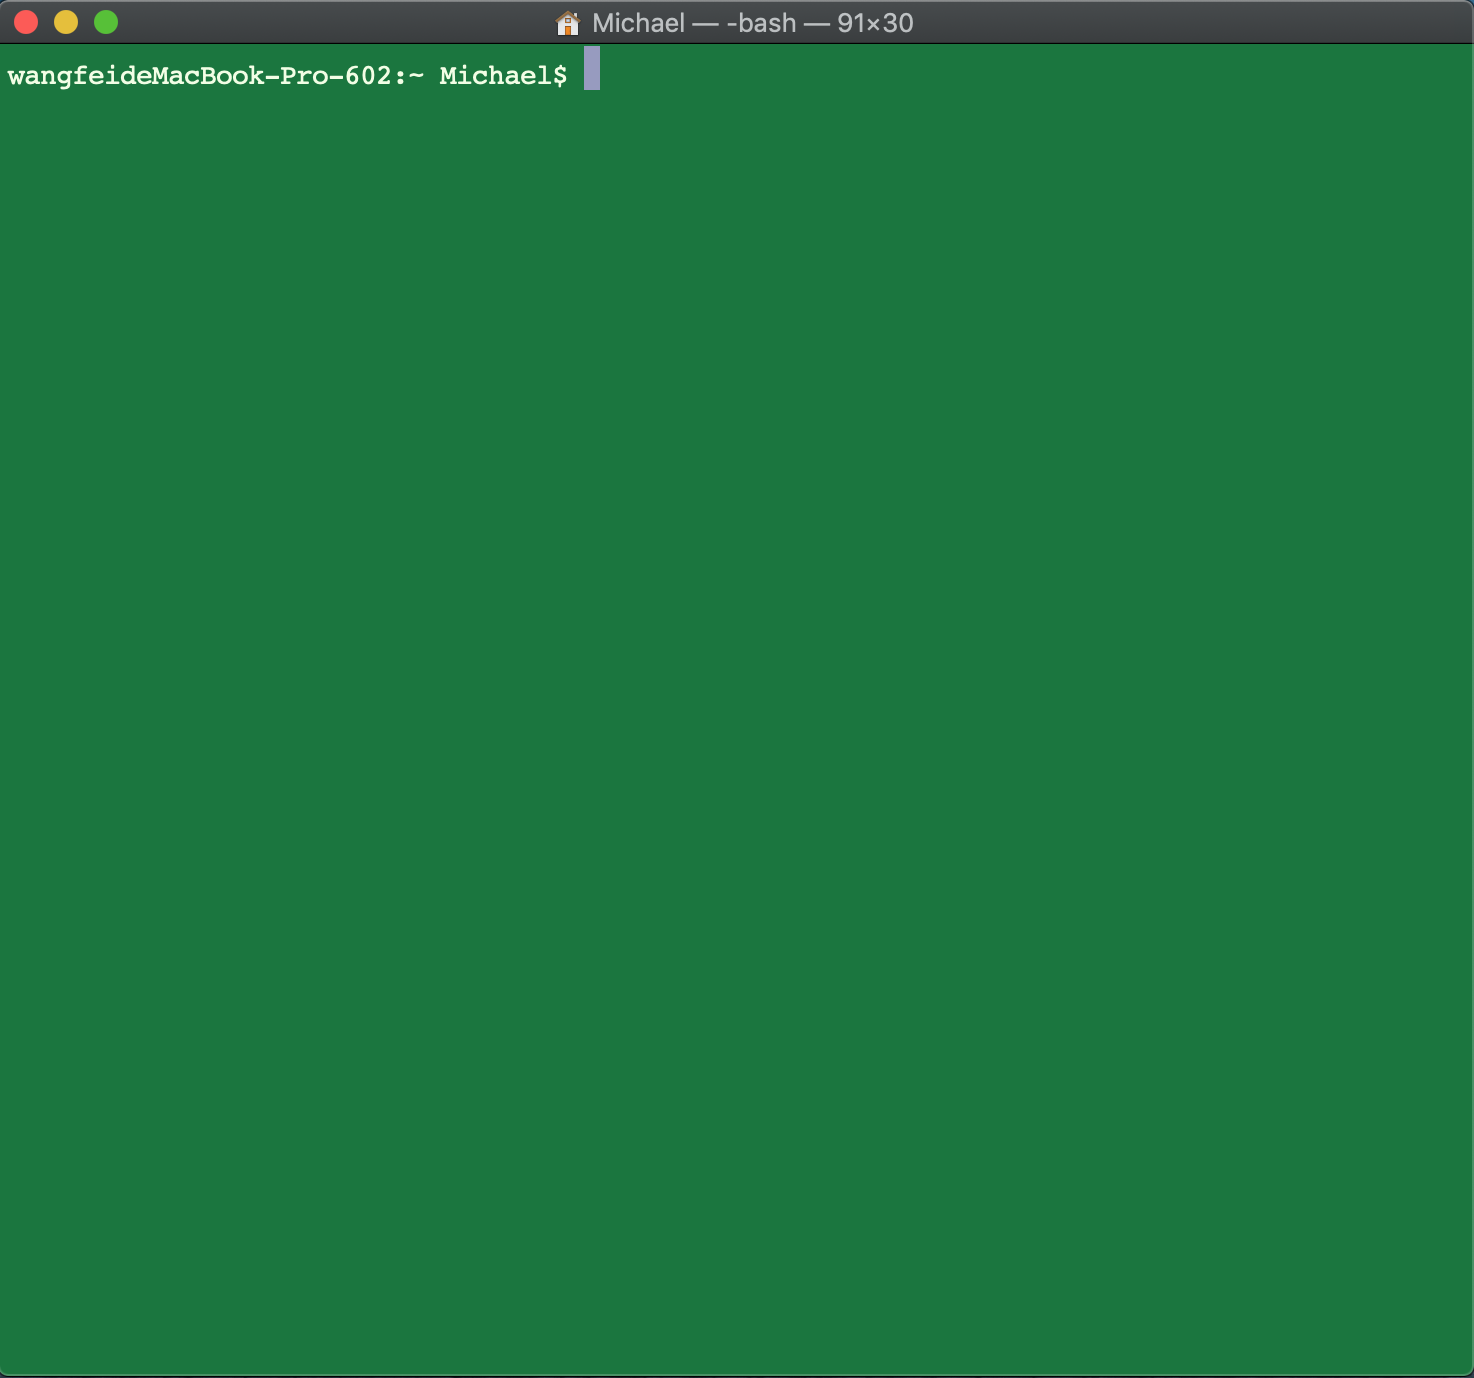
\includegraphics[width = 0.5\textwidth]{Pictures/terminal2}
		\caption{Terminal on Mac}
	\end{figure}
\end{frame}

\begin{frame}{Sooner or later, you will be on Github}
\begin{itemize}
\setlength\itemsep{1em} 
	\item GitHub is a web-based hosting service for version control using Git. It is mostly used for computer code. It offers all of the distributed version control and source code management functionality of Git as well as adding its own features.
	\item Here is the video link where I learned how to use Github: \begin{itemize} 
	\item A Youtube Video - \href{https://www.youtube.com/watch?v=0fKg7e37bQE&fbclid=IwAR3qiy3lyLxkwiE_6recElswiRJsknhFnnhjK5M4OMNkzBbI2aco01fJBOo}{click me \Coffeecup }
	\end{itemize}
	\item Github can be used to impress some girls when you go to a pub. 
\end{itemize}
\end{frame}

\begin{frame}{Essential Git Command}
\begin{table}[H]
	\centering
	\begin{tabular}{lcc}
	\hline 
	\hline 
		Command & Function & Tips \\
		\hline 
		\texttt{git clone} & clone cloud file to local directory & \\
		\texttt{git add} & add local file to cloud & \texttt{git add .(-A)} \\
		\texttt{git commit -m} & commit the message & \\
		\texttt{git push} & begin to upload & \\
		\texttt{git pull} & download from branch or cloud & \\
		\hline  
	\end{tabular}
\end{table}
	
\end{frame}


\section{IDE}

\begin{frame}{IDE:Integrated development environment}
	An integrated development environment is a software application that provides comprehensive facilities to computer programmers for software development. An IDE normally consists of 
	\begin{itemize}
	\setlength\itemsep{1em}
		\item a source code editor
		\item build automation tools
		\item a debugger
	\end{itemize} 
We will focus on building up a IDE for Python. For R, I suggest to download Rstudio. For matlab, you will install IDE directly when you install the programming. 
\end{frame}

\begin{frame}{Python IDE: Atom}
	Atom is a free and open-source text and source code editor for macOS, Linux, and Microsoft Windows with support for plug-ins written in Node.js, and embedded Git Control, developed by GitHub. Atom is a desktop application built using web technologies. Useful guides:
	\begin{itemize}
		\item A short intro on Atom:\href{https://blog.atom.io/2017/09/12/announcing-atom-ide.html}{click me \Coffeecup}
	\end{itemize}
Essential Packages:
\begin{itemize}
	\item \texttt{platformio-ide-Terminal}
	\item \texttt{atom-beautify}
	\item \texttt{atom-ide-ui}
	\item \texttt{build-python}
	\item \texttt{autocomplete-python}
	\item \texttt{hydrogen-launcher}
	\item \texttt{ide-python}
	\item \texttt{kite}
	\item \texttt{script}
\end{itemize}
\end{frame}

\begin{frame}{Why Atom ?}
	\begin{itemize}
	\setlength\itemsep{1em}
		\item Simple 
		\item Elegant 
		\item Beautiful
		\item Efficient
		\item Compact
	\end{itemize}
\end{frame}

\section{Which Language Should I pick up?}

\begin{frame}{Python, R, Julia and Matlab}
	\begin{itemize}
		\item R - Clean and tidy the data; Statistical modeling
		\item Python - Scientific Programming 
		\item Matlab/Julia - Numerical operation
	\end{itemize}
\begin{table}
	\centering
	\begin{tabular}{llcc}
	\toprule 
	Algorithm	& Programming & Running time & Using local memory \\
	\hline 
		&\texttt{Matlab} & 40.0244 seconds & relative high (4.92 GB)\\
		No &\texttt{Python} & 57 - 61.459 seconds & relative low (1 GB)\\
		&\texttt{Julia} & 80 seconds & relative low \\
		& \texttt{R} & & relative high\\
		\hline 
		& \texttt{Matlab} & 3.7044 seconds & \\
	Yes & \texttt{Python} & 5.4389 seconds & \\
	    & \texttt{Julia} & around 2 seconds & \\
	    & \texttt{R} & \\
	    \hline 
	    \hline 
	\end{tabular}
	\caption{Comparison for solving RBC model numerically with different programming}
\end{table}
\end{frame}

\begin{frame}{Which language should I use?}

	I have been struggling with this question for a while. After gaining some experiences on all those languages, here is my final call:
	\begin{itemize}
	\setlength\itemsep{1em}
		\item I will stick to Rstudio for data analyzing and calling statistical models (e.g. VAR, Bayesian Inference) 
		\item I will use Python to do mathematical programming and numerical operations as it is efficient
		\item I will try to use Matlab as little as possible for not breaking my laptop 
		\item Give up Julia temporarily and wait for the stable version
	\end{itemize}
\end{frame}

\section{Reference}

\begin{frame}{Book Recommendation}

To prepare this lecture, I have used this book:
\begin{itemize}
	\item \bibentry{paarsch2016gentle}
\end{itemize}

\end{frame}


\begin{frame}[allowframebreaks]{Reference}
\bibliographystyle{apalike}
\bibliography{IntroCom.bib}	
\end{frame}





	
\end{document}
